%%%%%%%%%%%%%%%%%%%%%%%%%%%%%%%%%%%%%%%%%
% University Assignment Title Page 
% LaTeX Template
% Version 1.0 (27/12/12)
%
% This template has been downloaded from:
% http://www.LaTeXTemplates.com
%
% Original author:
% WikiBooks (http://en.wikibooks.org/wiki/LaTeX/Title_Creation)
%
% License:
% CC BY-NC-SA 3.0 (http://creativecommons.org/licenses/by-nc-sa/3.0/)
% 
% Instructions for using this template:
% This title page is capable of being compiled as is. This is not useful for 
% including it in another document. To do this, you have two options: 
%
% 1) Copy/paste everything between \begin{document} and \end{document} 
% starting at \begin{titlepage} and paste this into another LaTeX file where you 
% want your title page.
% OR
% 2) Remove everything outside the \begin{titlepage} and \end{titlepage} and 
% move this file to the same directory as the LaTeX file you wish to add it to. 
% Then add \documentclass[12pt]{article}
\usepackage[english]{babel}
\usepackage{amsmath}
\usepackage{graphicx}
\usepackage{textcomp}
\usepackage{parskip}
\usepackage[colorinlistoftodos]{todonotes}
\usepackage{csquotes}
\usepackage{float}
\usepackage[backend=biber,style=ieee]{biblatex}
\addbibresource{bibliography.bib}

\begin{document}

\begin{titlepage}

\newcommand{\HRule}{\rule{\linewidth}{0.5mm}}
\center 

\textsc{\LARGE Iowa State University }\\[1.5cm] 
\textsc{\Large Center for Statistics and Applications in Forensic
Evidence
}\\[0.5cm] 

\HRule \\[0.4cm]
{ \huge \bfseries Shoe Print Data Collection: Additional Methods }\\[0.4cm] 
\HRule \\[1.5cm]



\begin{center}
\centering
 
\includegraphics[scale=.4]{csafe-logo}\\[1cm]
\end{center}







\end{titlepage}

\section{Introduction}

 When developing the methodology for the longitudinal shoe study conducted by the Center for Statistics and Applications in Forensic Evidence (CSAFE), collection procedures were designed to obtain the most ideal shoe-sole impression possible. While these images will be useful to the researcher and practitioner communities, they do not provide realistic examples of prints that would be collected from a crime scene/suspected crime scene. For this reason, CSAFE researchers have compiled this manual which contains procedures for further data collection and offers new, or edited, procedures that better represent the practices of current forensic examiners and crime scene teams. If at any time there is a question on any of these procedures, please make a note using a post-it note and e-mail the principal investigator, the project manager, the faculty in charge of the study, or the author of the specific procedure. 

\end{document} to your LaTeX file where you want your
% title page.
%
%%%%%%%%%%%%%%%%%%%%%%%%%%%%%%%%%%%%%%%%%
%\title{Title page with logo}
%----------------------------------------------------------------------------------------
%	PACKAGES AND OTHER DOCUMENT CONFIGURATIONS
%----------------------------------------------------------------------------------------

\documentclass[12pt]{article}
\usepackage[english]{babel}
\usepackage[utf8x]{inputenc}
\usepackage{amsmath}
\usepackage{graphicx}
\usepackage[colorinlistoftodos]{todonotes}

\begin{document}

\begin{titlepage}

\newcommand{\HRule}{\rule{\linewidth}{0.5mm}} % Defines a new command for the horizontal lines, change thickness here

\center % Center everything on the page
 
%----------------------------------------------------------------------------------------
%	HEADING SECTIONS
%----------------------------------------------------------------------------------------

\textsc{\LARGE Iowa State University}\\[1.5cm] % Iowa State University 
\textsc{\Large CSAFE}\\[0.5cm] % CSAFE
\textsc{\large Center for Statistics and Applications in Forensic Evidence }\\[0.5cm] % Center for Statistics and Applications in Forensic Evidence 

%----------------------------------------------------------------------------------------
%	TITLE SECTION
%----------------------------------------------------------------------------------------

\HRule \\[0.4cm]
{ \huge \bfseries EPSON Bed Scanner: Procedure }\\[0.4cm] % Title of your document
\HRule \\[1.5cm]
 
%----------------------------------------------------------------------------------------
%	AUTHOR SECTION
%----------------------------------------------------------------------------------------

\begin{minipage}{0.4\textwidth}
\begin{flushleft} \large
\emph{Author:}\\
James \textsc{E. Kruse} % Your name
\end{flushleft}
\end{minipage}
~
\begin{minipage}{0.4\textwidth}
\begin{flushright} \large
\emph{Supervisor:} \\
Dr. Guillermo \textsc{Basulto-Elias} % Supervisor's Name
\end{flushright}
\end{minipage}\\[2cm]

% If you don't want a supervisor, uncomment the two lines below and remove the section above
%\Large \emph{Author:}\\
%John \textsc{Smith}\\[3cm] % Your name
%----------------------------------------------------------------------------------------
%	LOGO SECTION
%----------------------------------------------------------------------------------------


\includegraphics[scale=.5]{Logo}\\[1cm]

\begin{center}
\begin{tabular}{ c   |   c } 
 
\end{tabular}
\end{center}
%----------------------------------------------------------------------------------------
%	DATE SECTION
%----------------------------------------------------------------------------------------

{\large \today}\\[2cm] % Date, change the \today to a set date if you want to be precise


 
%----------------------------------------------------------------------------------------

\vfill % Fill the rest of the page with whitespace

\end{titlepage}


\section{Introduction}

This is a continuation of the Paper Print/Vinyl Print Procedure and the Film Print Procedure. The following is the recommended procedure for using the EPSON Bed Scanner to scan paper and film prints. You will not need to bring up a program. By scanning a document, the bed scanner will bring up the program it requires.

\subsection{Procedure}

1. To scan the film and paper shoe prints into the computer, begin by logging in and turning on the scanner itself (Figure 1). 

\begin{figure}[!htp]
\centering
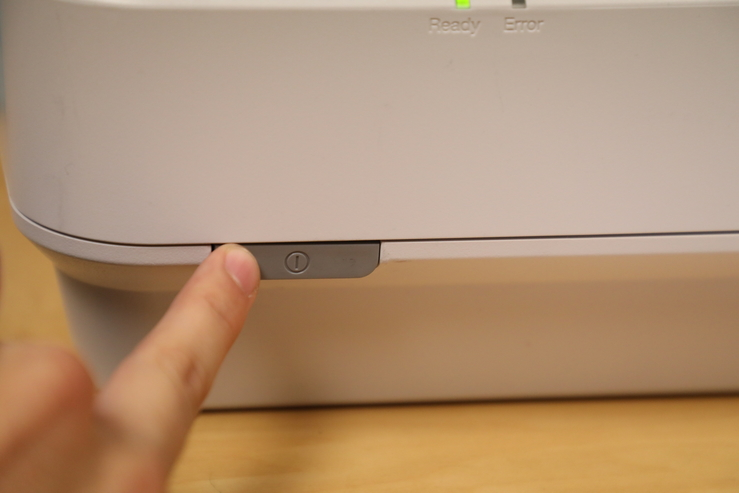
\includegraphics[scale=0.4]{Bed_On}
\caption{Switch on the power for the scanner.}
\label{Image 1}
\end{figure}

2. Open the lid of the scanner and place the print on the glass bed. The top left corner of the print, the end with the toe, needs to be placed in the back left corner of the bed (Figure 2). 

\begin{figure}[!htp]
\centering
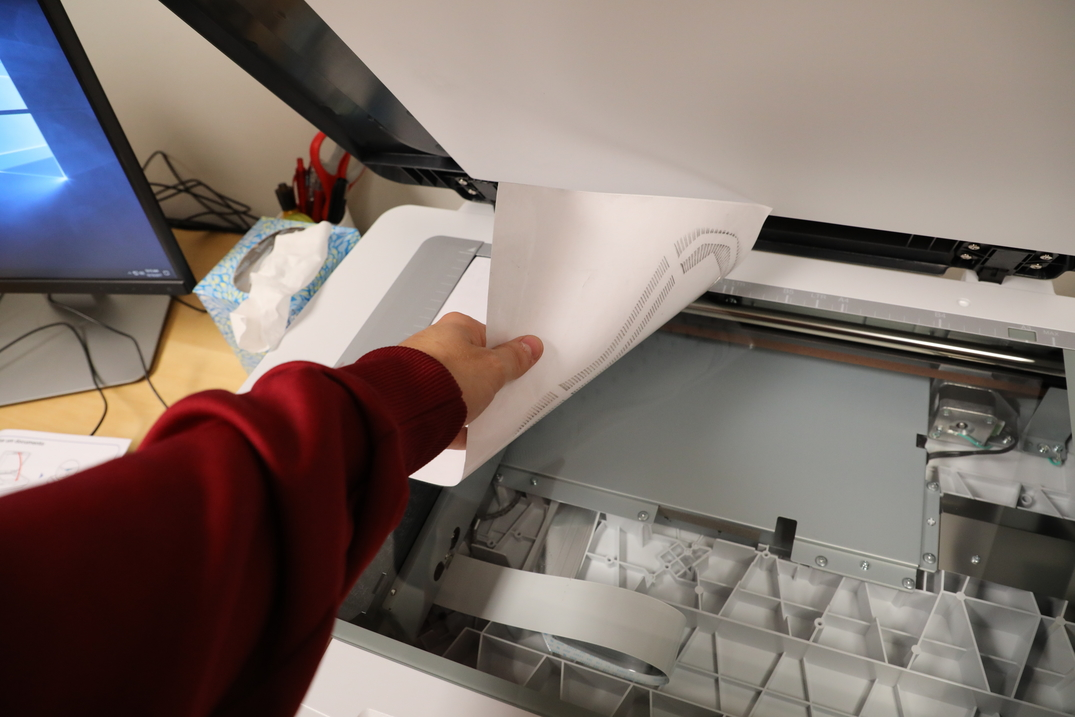
\includegraphics[scale=0.25]{Bed_Paper}
\caption{Place the print in the back left corner of the bed.}
\label{Image 2}
\end{figure}

\newpage

3. Close the lid and press the "scan" button on the bed scanner. This will bring up the program on the computer screen (Figure 3). 

\begin{figure}[!htp]
\centering
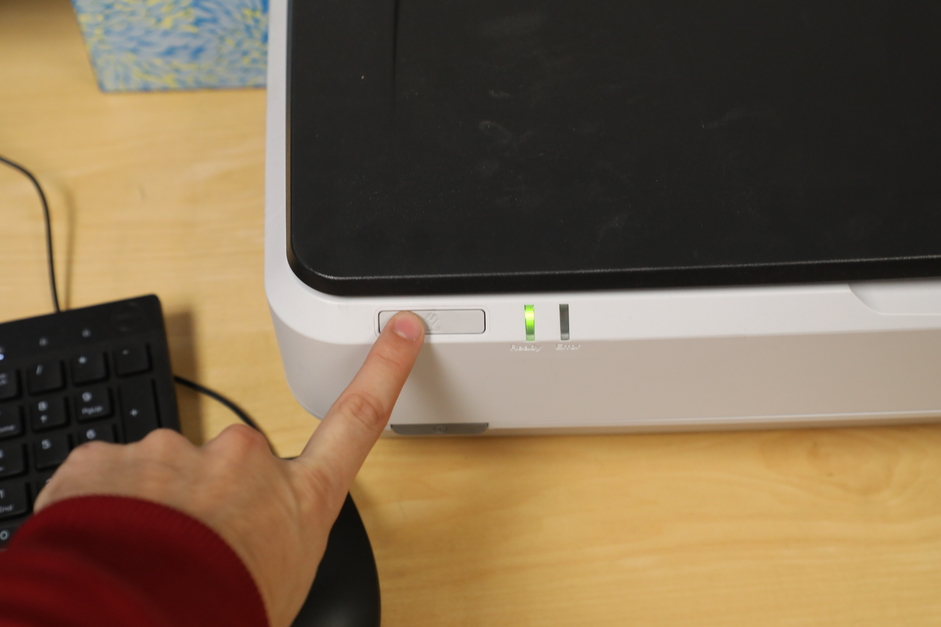
\includegraphics[scale=0.3]{Bed_Scan}
\caption{Press the Scan button.}
\label{Image 3}
\end{figure}


\newpage

4. The image that was generated will be a preview. Make sure that all settings are identical to those in figure four. The drop down menu above the image should be set to "normal". The final scan location will very depending on the cohort and collection. 

\begin{figure}[!htp]
\centering
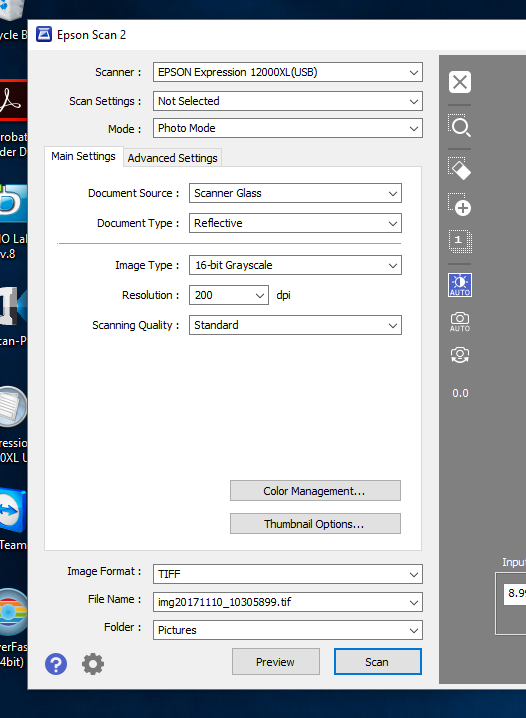
\includegraphics[scale=1.5]{Bed_Screen_1}
\caption{Settings for each scan. Make sure that all settings are identical to this image.}
\label{Image 4}
\end{figure}

\newpage

5. Dashed lines will appear around the image. Using the mouse, the dashed lines need to perfectly frame the image. This will auto crop this and all subsequent images during this sitting. Alterations may be necessary if a paper print is not square in the film or when changing to film (or vise versa). Always set dashed lines to the outside of the paper or film.

Note: When scanning film prints, the stapled tag must be folded over the back of the print. If not done, the shoe print will be covered in the scan. 

6.  All Files NEED to be saved as Tiff Files. For the full naming procedure, please refer to the inside cover of this manual and use the tool created by IT. 



7. Select preview at the bottom of the gray box and it will generate a sample of the scan (Figure 5-6). 

\begin{figure}[!htp]
\centering
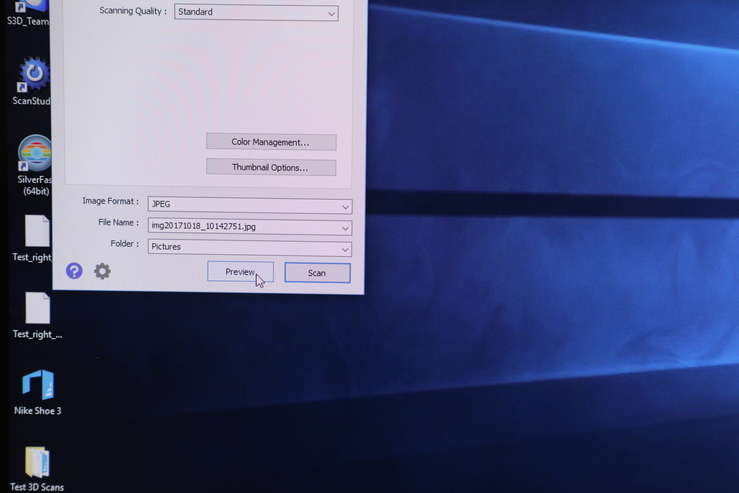
\includegraphics[scale=0.5]{Bed_Screen_4}
\caption{Conduct a pre-view scan.}
\label{Image 5}
\end{figure}

\begin{figure}[!htp]
\centering
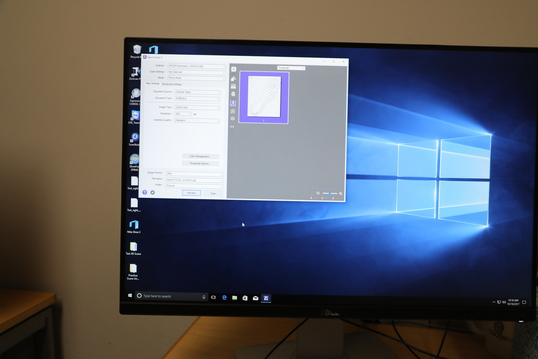
\includegraphics[scale=0.5]{Bed_Screen_5}
\caption{Sample of a pre-view scan.}
\label{Image 6}
\end{figure}

\newpage

8. If the crop is correct and the settings are right, press "scan" at the bottom of the gray box. This will scan the document and send it to the desired location. Figures 7 and 8 are examples of successful scans. 

\newpage

\begin{figure}[!htp]
\centering
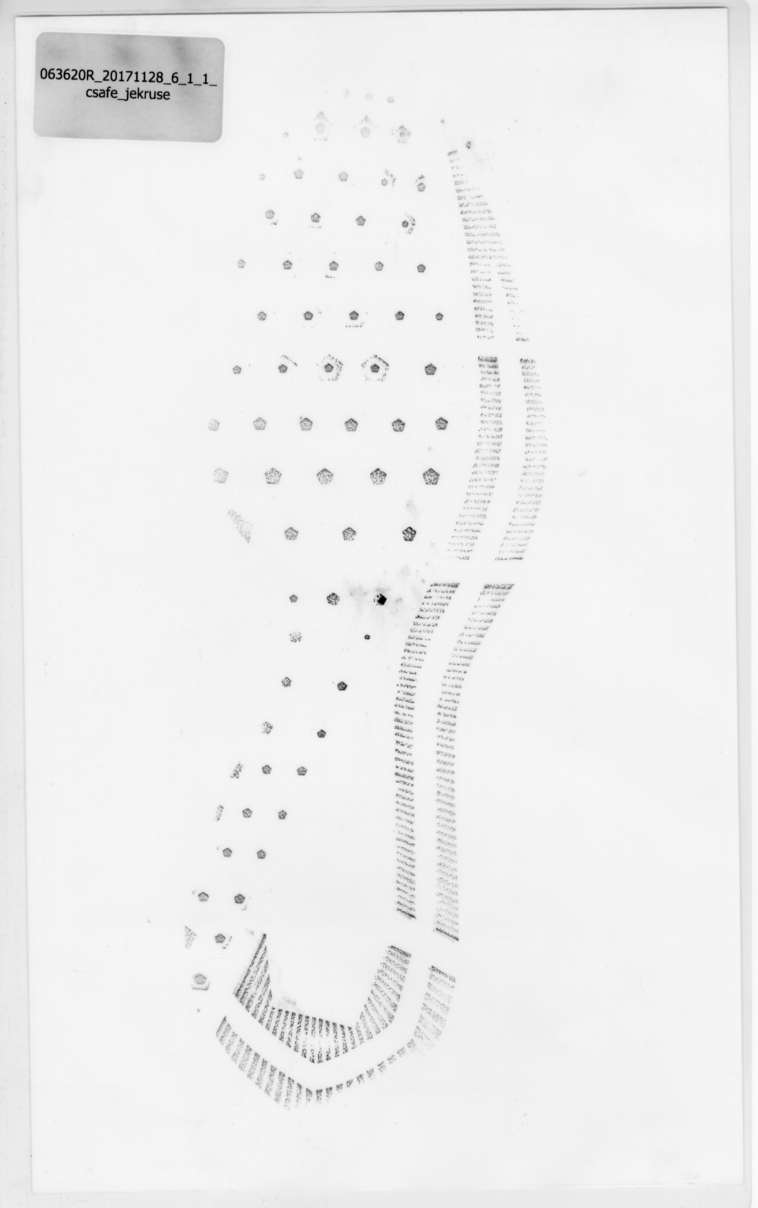
\includegraphics[scale=0.2]{Baseline_Paper_1}
\caption{Sample of a proper paper print scan}
\label{Image 7}
\end{figure}

\begin{figure}[!htp]
\centering
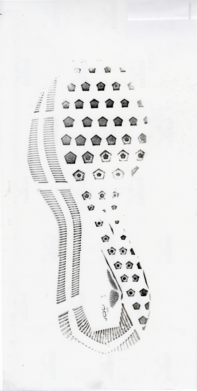
\includegraphics[scale=2]{New_Film}
\caption{Sample of a proper film print scan}
\label{Image 8}
\end{figure}

9. Continue to scan the remainder of the prints while making sure to change the crop as needed. See figures 7 and 8 for examples of proper scans. 



\end{document}